\documentclass[sigconf, review, anonymous]{acmart}
\usepackage{graphicx}
\usepackage{multirow}
\usepackage{booktabs}
\usepackage{array}
\usepackage{tabularx}
\usepackage{xcolor}
\usepackage{enumitem}
\usepackage{subcaption}
\usepackage{balance}
\usepackage{listings}
\usepackage{pgfplots}
\pgfplotsset{compat=1.18}
\usepackage{pgf-pie}
\usepackage{xspace}
\usepackage{amsmath}
\usepackage{seqsplit}
\usepackage{tcolorbox}
\tcbuselibrary{breakable, skins}
\usepackage{url}
\usepackage{placeins}

\newcommand{\tool}{\textsc{PaiChecker}\xspace}
\newcommand{\ie}{\textit{i.e.}\xspace}
\newcommand{\eg}{\textit{e.g.}\xspace}
\newcommand{\etal}{\textit{et al.}\xspace}
\newcommand{\todo}[1]{\textcolor{red}{\textbf{[TODO: #1]}}}
\newcommand{\finding}[1]{\vspace{0.3em}
\noindent
\fbox{\parbox{0.96\columnwidth}{\textbf{Finding:} #1}}
\vspace{0.3em}}

\lstset{ basicstyle=\ttfamily\small, breaklines=true, frame=single, numbers=left,
numberstyle=\tiny
\color{gray}
, xleftmargin=2em, framexleftmargin=1.5em, backgroundcolor=
\color{gray!5}
, captionpos=b }

\title{\tool: Uncovering and Checking PR-Issue Misalignment
in SWE-Bench-Like Benchmarks}

\author{Anonymous Authors}

\begin{document}
    \begin{abstract}
  %     SWE-bench-like benchmarks are a family of benchmarks for
  % evaluating LLMs on automated issue resolution. They typically follow a common construction pipeline: each PR (Pull Request) is paired with its linked issue by extracting issue references from the PR description; the issue description is used as the problem statement, and the PR patch serves as the test oracle. However, due to the
  % inherent complexity of developing and maintaining large
  % repositories, such PR-Issue pairings are often misaligned in practice. While prior work has identified several quality issues in SWE-bench, these efforts target                                      
  % individual benchmarks and overlook this systematic construction-level                                       
  % problem prevalent across most SWE-bench-like benchmarks. In this work, we systematically study all 500 SWE-bench Verified instances, finding    
  % that 13.6\% exhibit misalignment across five patterns and eleven fine-grained scenarios.  To detect and
  % categorize such misalignment at scale, we propose \tool, a novel multi-agent system for checking PR-Issue misalignment in SWE-bench-like benchmarks. Guided by a \textit{text-driven, code-validation} principle, \tool adopts a three‑phase design that combines specific pattern identification, cross-agent label synthesis, and code-level validation, thereby enabling more accurate, generalizable, and progressively verified detection.                               
  % Experiments on the SWE-Gym dataset demonstrate the effectiveness of \tool: it achieves the best 
  % performance across all four LLM backbones, reaching up to 92.12\% binary     
  % accuracy and 84.66\% exact match, outperforming the strongest baseline by      
  % 5.1--12.4 and 8.6--17.8 percentage points, respectively. All annotated data and tools are publicly available.

        SWE-bench-like benchmarks are widely-used for
  evaluating LLM's issue resolution capability. They typically follow a common construction pipeline: each PR (Pull Request) is paired with its linked issue by extracting issue references from the PR description; the issue description is used as the problem statement, and the PR patch serves as the test oracle. However, due to the
  inherent complexity of developing and maintaining large
  repositories, such PR-Issue pairings are often misaligned in practice.
  % While prior work has identified several quality issues in SWE-bench, these efforts target individual benchmarks and overlook this systematic construction-level problem prevalent across most SWE-bench-like benchmarks.
  In this work, we systematically study SWE-bench Verified instances, finding    
  that 13.6\% exhibit misalignment across five patterns in eleven fine-grained scenarios. To enable reliable and scalable construction of those benchmarks in the future, we propose \tool, a multi-agent system for checking PR-Issue misalignment in SWE-bench-like benchmarks. Guided by a \textit{text-driven, code-validation} principle, \tool adopts a three‑phase design that combines specific pattern identification, cross-agent label synthesis, and code-level validation, thereby enabling more accurate, generalizable, and progressively verified detection.                               
  Experiments on the SWE-Gym dataset demonstrate the effectiveness of \tool: it achieves the best 
  performance across all four LLM backbones, reaching up to 92.12\% binary     
  accuracy and 84.66\% exact match, outperforming the strongest baseline by      
  5.1--12.4 and 8.6--17.8 percentage points, respectively.
  % All annotated data and tools are publicly available.
    
    \end{abstract}

    \maketitle

    %% ============================================================
    %% SECTION 1: INTRODUCTION
    %% ============================================================
    \section{Introduction}
    \label{sec:intro}

    The emergence of large language models (LLMs) capable of code generation and
    program repair has spurred the need for rigorous, real-world benchmarks~\cite{swebench,
    jain2024livecodebenchholisticcontaminationfree, he2025sweperf,xu_aligning_2025, deng2025swepro}. Among them, SWE-bench~\cite{swebench} has become one of the most influential benchmarks for evaluating LLMs on automated issue solving tasks~\cite{team_trae_2025,xia_agentless_2024,minisweagent,zhang_autocoderover_2024, yang_kimi-dev_2025}. SWE-bench constructs task instances from real-world
    GitHub repositories, using issue descriptions as problem statements and the corresponding pull request (PR) patches as test oracles. Following its success, several SWE-bench-like
    benchmarks have emerged to address various limitations, an non-exhaustive list includes SWE-bench
    Verified~\cite{swebenchverified}, SWE-Gym~\cite{swegym}, SWE-PolyBench~\cite{swepoly}, SWE-Smith~\cite{swesmith}, and SWE-Bench-Live~\cite{swebenchlive}. These benchmarks largely adopt the same construction
    pipeline: they filter PRs by quality criteria, then use
    regular expressions to extract linked issues from PR descriptions,
    forming PR-Issue pairs as task instances.

    However, this construction pipeline rests on a critical
    % yet largely unexamined
    assumption: that each PR is \textit{well-aligned} with its linked issue, i.e.,
    the PR exclusively and completely addresses the stated problem,
    and the issue fully specifies what the PR solves. In
    practice, this assumption is frequently violated. A PR may bundle fixes for
    multiple issues, serve as a follow-up to a previous incomplete
    fix, introduce new defects alongside the intended fix, or implement details clarified only in later discussions rather than the original description.
    Such misalignment renders the benchmark instance problematic:
    \textit{the problem statement may not fully describe the expected solution, or the test
    oracle may evaluate aspects unrelated to the stated problem}, directly
    undermining evaluation fairness and reliability.

In this paper, we present a systematic study of \textit{PR-Issue misalignment} in SWE-bench-like benchmarks, where \textit{PR-Issue misalignment} refers to discrepancies between a \textit{pull request code implementation} and the \textit{issue description} it is linked to in the dataset.
We manually analyze all 500 instances in SWE-bench Verified~\cite{swebenchverified} and find that 13.6\% exhibit misalignment. We further classify these misalignments into five patterns spanning 11 fine-grained scenarios. To quantify the impact of misalignment, we correlate it with agent resolution rates and find that 41.2\% of instances never resolved by any of the 131 leaderboard agents are misaligned, suggesting that a substantial portion of unsolved tasks may stem from flawed benchmark construction rather than genuine engineering difficulty.

These findings motivate the need for automated detection and categorization of PR–Issue misalignment at scale. However, detecting misalignment directly from the code implementation and issue description is challenging, as the intent reflected in code is inherently ambiguous. This ambiguity arises from the nature of code changes: in complex cases, the intended behavior may depend on modifications spanning hundreds or thousands of lines, while in simpler cases, the implemented behavior may still be incomplete or defective. 
In contrast, PR-side textual artifacts, such as PR descriptions and discussions, explicitly express intent and are naturally comparable to issue descriptions, as both are written in natural language and share a common semantic structure; by contrast, code primarily captures implementation details rather than intent. This asymmetry between textual artifacts and code motivates the key design principle of our approach, namely the \textit{text-driven, code-validation} principle, which first assesses alignment based on textual evidence and then validates it against code.
 
According to this principle, the task is well suited to LLM reasoning and tool-augmented agents, because it is fundamentally a semantic comparison task. We therefore adapt Mini-SWE-Agent~\cite{minisweagent}, augmenting it with task-specific prompts and GitHub API access, as a representative general-purpose agent baseline. However, this approach has three limitations:~(1) it lacks specialization: different misalignment patterns require different inputs and reasoning workflows, but a single prompt conflates these heterogeneous requirements and often misses subtle yet critical evidence. ~(2) it has limited generalizability: when no predefined pattern applies, it tends to force-fit the instance into the nearest known category, even though real-world misalignments often fall outside the taxonomy. ~(3) it lacks verification machanism: its predicted label may not match its own textual reasoning as well as the code implementation. We illustrate these limitations in detail in Section~\ref{sec:motivation}.

To address these limitations, we propose \tool
(\textbf{P}R-\textbf{I}ssue \textbf{A}lignment Checker), a
three-phase multi-agent framework guided by a
\textit{text-driven, code-validation} principle. The first two
phases focus on textual analysis, and the third performs
code-level verification. Specifically, Phase I addresses
limitation(1) through three specialized subagents, each with a
focused artifact subset and tailored workflow. Phase II addresses limitation(2) via a coordinator that synthesizes cross‑subagent evidence to identify misalignment beyond known patterns. For limitation(3), \tool introduces a two-level
\textit{self-correction} mechanism: PhaseII re-verifies each
label against its textual evidence, and Phase~III validates it
against the actual code implementation.                                               

    We evaluate \tool on SWE-gym~\cite{swegym},
    comparing it against four baselines including zero-shot prompting~\cite{zeroshot_fewshot}, few-shot prompting~\cite{zeroshot_fewshot},
    chain-of-thought prompting~\cite{cot}, and Mini-SWE-Agent~\cite{minisweagent}. Using
    four state-of-the-art LLMs as backbones (GPT-5.3 Codex~\cite{gpt53codex}, Qwen-3.5 Plus~\cite{qwen35},
    Gemini-3.1-Pro Preview~\cite{gemini31pro}, and Claude-Sonnet-4.6~\cite{claudesonnet46}), \tool achieves the best 
  performance across all four LLM backbones, reaching up to 92.12\% binary     
  accuracy and 84.66\% exact match, outperforming the strongest baseline by      
  5.1--12.4 and 8.6--17.8 percentage points. Ablation studies confirm each component's                          
  contribution.

    In summary, this paper makes the following contributions:
\begin{itemize}[leftmargin=*]
      \item \textbf{Problem Formulation.} We identify PR-Issue                          
          misalignment as a systematic construction problem in                       
          SWE-bench-like \nolinebreak bench\nolinebreak marks.
                                                                                           
      \item \textbf{Empirical Study.} We analyze all 500 SWE-bench                       
          Verified instances, deriving a taxonomy of five patterns with                    
          11 scenarios and finding 13.6\% misaligned                                       
          (Section~\ref{sec:preliminary}).                                                 
   
      \item \textbf{Detection Framework.} We propose \tool, a                              
          multi-agent framework for automated detection and                              
          categorization of PR-Issue misalignment
          (Section~\ref{sec:method}).
                                                                                           
      \item \textbf{Evaluation.} Experiments on SWE-Gym with four
          state-of-the-art LLMs demonstrate the effectiveness of \tool.
          (Sec\nolinebreak tions~\ref{sec:results}).
                                                                                           
      \item \textbf{Data Availability.} We release all annotated data                     
          and \tool to support future benchmark
          curation\footnote{Data and tools available at:                                   
          \url{https://anonymous.4open.science/r/PAIChecker-FF08}. We also provide the code and data in the supplementary material in case the link is unavailable due to website instability.}                       
  \end{itemize}


    %% ============================================================
    %% SECTION 2: PRELIMINARY STUDY
    %% ============================================================
    \section{Preliminary Study and Motivation}
    \label{sec:preliminary} In this section, we systematically investigate the
    existence, prevalence, and impact of PR-Issue misalignment in SWE-bench-like
    benchmarks. Our findings provide the empirical foundation and motivation for
    our automated misalignment checker \tool. This study focuses on two research
    questions:
    \begin{itemize}[leftmargin=*]
        \item \textbf{RQ1 (Taxonomy and Prevalence):} What are the types of PR-Issue
            misalignments, and how prevalent are they?

        \item \textbf{RQ2 (Impact):} How does PR-Issue misalignment affect agent
            evaluation reliability?
    \end{itemize}

    \subsection{Study Design}
    \label{sec:study_design}

    \subsubsection{Dataset}
    \label{sec:study_dataset} We conduct our study on SWE-bench Verified~\cite{swebenchverified},
  a human-validated subset of 500 SWE-Bench~\cite{swebench} instances.                     
  We select it for two reasons: (1)~its human validation represents a                      
  high-quality baseline, so misalignments found here likely reflect                        
  broader issues in other SWE-bench-like benchmarks; (2)~its official                      
  experiments repository~\cite{sweexperiments} provides per-instance                       
  resolution data for 131 leaderboard agents, enabling quantitative                        
  analysis for RQ2.

    \subsubsection{Method}
    \label{sec:study_method}

    \textbf{Manual Examination Process.}\quad Following established                          
  practices in qualitative SE research~\cite{groundedref1,                               
  groundedref2}, we apply open coding~\cite{opencoding} to derive a
  misalignment taxonomy (RQ1). First, we collect per instance: issue-side
  artifacts (description, discussion), PR-side artifacts (description,                     
  discussion, code review, commits, changed files), and cross-reference
  metadata. Then, we code all 500 instances, iteratively grouping codes                     
  into higher-level categories to form a draft taxonomy; a single                        
  instance may exhibit multiple patterns. Last, the draft taxonomy was                           
  reviewed by the second author; disagreements were resolved with a
  third author until consensus.                                                                             
                                                                                           
  \textbf{Leaderboard Data Collection.}\quad To assess the impact of
  misalignment on evaluation reliability, we collect per-instance                    
  resolution data from the official SWE-bench experiments                                
  repository~\cite{sweexperiments}, recording per-instance resolution counts for 131 leaderboard agents. 

    \subsection{Results and Analysis}
    \label{sec:study_results}

    \subsubsection{RQ1: Taxonomy and Prevalence of Misalignment}
    \label{sec:rq1}
    
    Table~\ref{tab:misalignment_patterns} summarizes the taxonomy of five                    
  patterns with 11 fine-grained scenarios, with instance counts in parentheses. Our classification also follows the                  
  \textit{text-driven, code-validation} principle (Section ~\ref{sec:intro}). We elaborate on each pattern below. 


    \begin{table}[t]
        \centering
        \caption{Taxonomy of PR-Issue misalignment patterns in SWE-bench Verified (68/500 instances). Instances may exhibit multiple patterns.}
        \label{tab:misalignment_patterns}
        \footnotesize
        \begin{tabularx}{\columnwidth}{@{}>{\raggedright\arraybackslash}p{0.3\columnwidth}X@{}}
            \toprule
            \textbf{Pattern} & \textbf{Scenario} \\
            \midrule
            \multirow{4}{=}{\textbf{SC:} PR Scope Creep}
                & \textbf{SC-1\,(12):} Resolves multiple issues; only one specified \\
                & \textbf{SC-2\,(2):} Adds features beyond issue description \\
                & \textbf{SC-3\,(2):} Bundles fixes for bugs not in the issue \\
                & \textbf{SC-4\,(6):} Extra patches for other issues alongside fix \\
            \midrule
            \multirow{2}{=}{\textbf{DP:} Defective PR}
                & \textbf{DP-1\,(14):} Introduces new bugs requiring follow-up fixes \\
                & \textbf{DP-2\,(16):} Incomplete solution requiring follow-up \\
            \midrule
            \multirow{2}{=}{\textbf{IS:} Incomplete Specification}
                & \textbf{IS-1\,(12):} Details supplemented by reporter in discussion \\
                & \textbf{IS-2\,(6):} Addresses new problem from later discussion \\
            \midrule
            \multirow{2}{=}{\textbf{FP:} Follow-up PR}
                & \textbf{FP-1\,(2):} Fixes bugs introduced by a previous PR \\
                & \textbf{FP-2\,(1):} Supplements a prior PR \\
            \midrule
            \textbf{UL:} Unspecified Literal
                & \textbf{UL-1\,(1):} Asserts exact literals (\eg messages) not in issue \\
            \bottomrule
        \end{tabularx}
    \end{table}

    %-------------------------------------------------------------
    %  Reusable tiny-box style (defined once)
    %-------------------------------------------------------------
    \newcommand{\artifactlabel}[1]{%
      \noindent\textbf{\small #1}\vspace{2pt}\hrule\vspace{4pt}}


    %-------------------------------------------------------------
    %  SC / DP / FP / IS — double-column, four side by side
    %-------------------------------------------------------------
    \begin{figure*}[t]
    \captionsetup{justification=raggedright}
      \centering
      \begin{subfigure}[t]{0.235\textwidth}
        
\includegraphics[width=\textwidth]{fig_sc.pdf}
        \caption{SC(sphinx\-doc\_\_sphinx-10614): The PR closed three distinct issues; the problem statement covers only one. }
        \label{fig:sc1_example}
      \end{subfigure}
      \hfill
      \begin{subfigure}[t]{0.235\textwidth}
        
\includegraphics[width=\textwidth]{fig_dp.pdf}
        \caption{DP(sympy\_\_sympy-13852): The PR introduces random test failures that require a follow‑up fix.}
        \label{fig:dp_example}
      \end{subfigure}
      \hfill
      \begin{subfigure}[t]{0.235\textwidth}
        
\includegraphics[width=\textwidth]{fig_fp.pdf}
        \caption{FP(django\_\_django-12125): The PR addresses only the remaining bug not the full issue.}
        \label{fig:fp_example}
      \end{subfigure}
      \hfill
      \begin{subfigure}[t]{0.235\textwidth}
        
\includegraphics[width=\textwidth]{fig_is.pdf}
        \caption{IS(sympy\_\_sympy-20916):The issue is too vague, confusing even the maintainer, so the model likely won’t understand it either..}
        \label{fig:is_example}
      \end{subfigure}
      \caption{Examples of four misalignment patterns.}
      \label{fig:examples_4}
      \captionsetup{justification=centering} 
    \end{figure*}


  \textbf{PR Scope Creep (SC)} occurs when the PR delivers functionality                   
  beyond what the issue requests. We consider this a misalignment                          
  because it creates a mismatch between the task and its evaluation: the                   
  test patch validates requirements absent from the                                        
  \texttt{problem\_stateme-\allowbreak nt}, penalizing agents that correctly solve                      
  the stated problem. Specifically, SC-3 refers to pre-existing bugs in the repository, whereas SC-4 refers to patches addressing unrelated Issues.
  
  \emph{Example.} Figure~\ref{fig:sc1_example} shows
  \texttt{sphinx-doc\_\_sphinx-10614}: the \texttt{pro-\allowbreak blem\_statement}
  captures only issue \texttt{\#10570}, but the PR closes                     
  three distinct issues. An agent correctly resolving \texttt{\#10570} may still
  fail if it does not coincidentally address the two unstated issues. 


    \textbf{Defective PR (DP)} captures cases where the PR itself is flawed---introducing new bugs or providing an incomplete fix which requires subsequent corrective work. We consider this a type of misalignment because the test patch may encode buggy behavior as the expected output or validate only a partial solution.

    \emph{Example.} Figure~\ref{fig:dp_example} shows \texttt{sympy\_\_sympy-13852}. The PR fixes the reported issue but introduces random test failures, requiring a follow‑up fix. Yet the benchmark treats the original defective PR as ground truth.


\textbf{Follow-up PR (FP)} is the converse of DP: the PR supplements
  or fixes a previous PR for the same issue. We consider this a                         
  misalignment because the codebase already contains the earlier PR's                      
  changes, so the model benefits from prior work and the evaluation does
  not reflect its true capability. 

  \emph{Example.} Figure~\ref{fig:fp_example} shows                                        
  \texttt{django\_\_django\-12125}: a previous PR partially fixed the                      
  inner-class path issue for \texttt{Field} subclasses, but                                
  \texttt{Enum} serialization remained broken. The current PR addresses                  
  only that remaining gap; the codebase already contains the earlier                   
  fix.


\textbf{Incomplete Specification (IS)} occurs when the original issue
  description is supplemented or revised in later discussion. We
  consider this a misalignment because agents receive only the initial
  description, which in such cases lacks information needed for
  resolution. Following the standard bug report format, which includes
\textit{code to reproduce, actual behavior, and expected
behavior}~\cite{bettenburg_what_2008,issuetemp1,issuetemp2,issuetemp3,issuetemp4},
we distinguish two forms of incomplete specification, both grounded
in maintainer consensus. ~(1)The issue is \textit{incomplete} when a
maintainer explicitly requests a missing component, This type of misalignment resembles the "unspecified" criterion in SWE-bench-verified~\cite{annotation_instruction}, but is more objective: insufficiency is only flagged when the repository maintainer also fails to understand the issue. ~(2) The issue is
\textit{redefined} when a component is revised by maintainer
agreement (\eg the expected behavior). 
  
  \emph{Example.} Figure~\ref{fig:is_example} shows
  \texttt{sympy\_\_sympy-20916}: the original issue describes incorrect
  formatting and expected output, but lacks reproduction code. At a
  maintainer's request, the reporter supplies a Python script containing
  key information absent from the \texttt{problem\_statement}.

    \textbf{Unspecified Literal (UL)} occurs when the test patch asserts exact literal values (\eg exception messages) introduced by the PR but absent from the issue. We consider this a type of misalignment because it penalizes agents that produce semantically correct outputs differing in literal form. This reflects an overly strict test oracle that requires implementation-specific details unrecoverable from the issue description alone.

    \emph{Example.} \texttt{astropy\_\_astropy-13033}: the issue requests ``\textit{an exception that tells the user which required columns are actually missing}'' without specifying the exact wording. However, the test patch asserts the precise string \texttt{``TimeSeries object is invalid -- expected {[}'time',\,'a'{]} as the first columns but found {[}'time',\,'b'{]}''}, rejecting correct fixes with different wording.

    \finding{13.6\% (68/500) of SWE-bench Verified instances exhibit PR-Issue misalignment. Defective PR (44.1\%), PR Scope Creep (32.4\%), and Incomplete Specification (26.5\%) are the three most prevalent pattern families.}

    \subsubsection{RQ2: Impact on Evaluation Reliability}
    \label{sec:rq2}

    In this RQ, we aim to investigate the practical impact of PR-Issue misalignment. To answer this, we correlate the misalignment labels from Section~\ref{sec:rq1} with                     
  resolution outcomes of the 131 leaderboard                                               
  agents~\cite{sweexperiments}, recording for each instance how many                       
  agents successfully resolve it.                                                          
  Figure~\ref{fig:rq2_trend} visualizes the relationship.  


%-------------------------------------------------------------
%  RQ2 Trend Figure
%-------------------------------------------------------------
\begin{figure}[!t]
\centering
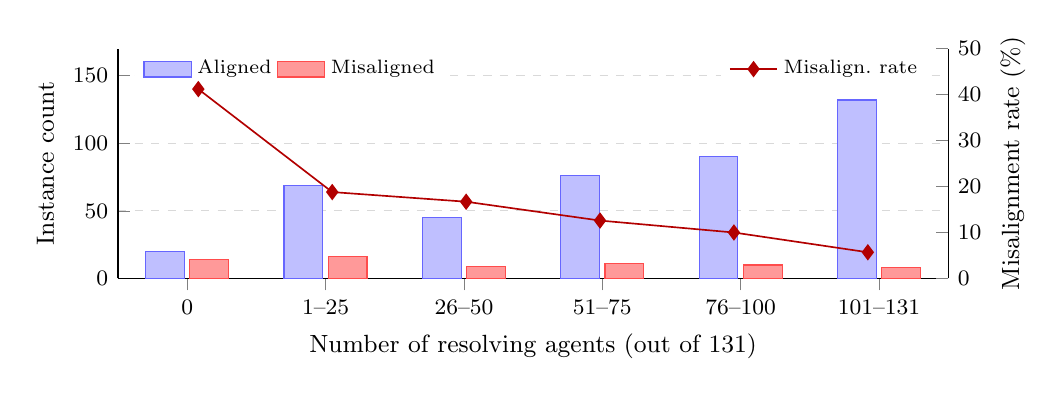
\begin{tikzpicture}
\begin{axis}[
    width=\columnwidth,
    height=4.5cm,
    ybar,
    bar width=14pt,
    xlabel={Number of resolving agents (out of 131)},
    ylabel={Instance count},
    ymin=0, ymax=170,
    xtick=data,
    xticklabels={0, 1--25, 26--50, 51--75, 76--100, 101--131},
    x tick label style={font=\footnotesize},
    y tick label style={font=\footnotesize},
    label style={font=\small},
    axis y line*=left,
    axis x line*=bottom,
    ymajorgrids=true,
    grid style={dashed, gray!30},
    legend style={at={(0.02,1)}, anchor=north west, font=\scriptsize, draw=none,legend columns=-1},
    area legend,
]
% Aligned instances (bars)
\addplot[fill=blue!25, draw=blue!60] coordinates {
    (1,20) (2,69) (3,45) (4,76) (5,90) (6,132)
};
\addlegendentry{Aligned}

% Misaligned instances (bars)
\addplot[fill=red!40, draw=red!70] coordinates {
    (1,14) (2,16) (3,9) (4,11) (5,10) (6,8)
};
\addlegendentry{Misaligned}
\end{axis}

% Overlay: misalignment rate line on right y-axis
\begin{axis}[
    width=\columnwidth,
    height=4.5cm,
    axis y line*=right,
    axis x line=none,
    ylabel={Misalignment rate (\%)},
    ylabel style={font=\small},
    ymin=0, ymax=50,
    ytick={0,10,20,30,40,50},
    y tick label style={font=\footnotesize},
    xtick=data,
    xticklabels={},
    xmin=0.4, xmax=6.6,
    legend style={at={(0.98,1)}, anchor=north east, font=\scriptsize, draw=none},
]
\addplot[color=red!70!black, mark=diamond*, semithick, mark size=2.5pt] coordinates {
    (1,41.2) (2,18.8) (3,16.7) (4,12.6) (5,10.0) (6,5.7)
};
\addlegendentry{Misalign.\ rate}
\end{axis}
\end{tikzpicture}
\caption{Misalignment rate decreases monotonically as instances are resolved by more agents. Bars show instance counts (left axis); the line shows the misalignment rate within each bucket (right axis). Among the 34 never-resolved instances, 41.2\% are misaligned, compared to only 5.7\% among instances solved by $>$100 agents.}
\label{fig:rq2_trend}
\end{figure}


    Among the 500 instances, 34 have never been resolved by any of the
  131 leaderboard agents. Of these, 14 (41.2\%) exhibit PR-Issue
  misalignment, suggesting that the hardest instances may challenge
  agents due to unstated evaluation requirements, not task complexity
  alone. More broadly, Figure~\ref{fig:rq2_trend} shows a monotonic
  decrease in misalignment rate as instances are resolved by more
  agents: from 41.2\% among never-resolved instances to 5.7\% for those
  resolved by over 100 agents. Well-aligned instances are solvable by
  many agents, whereas misaligned instances introduce extraneous
  difficulty that few agents overcome by coincidence. These findings are consistent with OpenAI's concurrent
  analysis~\cite{swebenchverifiednolonger}, though we arrive at a
  similar conclusion from a distinct perspective: systematic PR-Issue
  misalignment in benchmark construction.

      \finding{41.2\% of instances never resolved by any of the 131
  leaderboard agents exhibit PR-Issue misalignment. Misalignment rate
  decreases monotonically from 41.2\% (never-resolved) to 5.7\%
  (resolved by $>$100 agents), suggesting that misalignment may
  introduce non-engineering difficulty that distorts benchmark
  evaluations.}

        \begin{figure*}[t]
    \centering
    
\includegraphics[width=\textwidth]{motivation.pdf}
    \caption{Motivating Example \texttt{iterative\_\_dvc-4872}: PR~\#4872 is accidentally
    linked to issue~\#4796 but actually fixes issue~\#4504. Backbone:
    Gemini-3.1-Pro Preview. Mini-SWE-Agent and CoT force-classify as SC;
    \tool's coordinator correctly drops SC and assigns \textit{Others} by
    synthesizing suspicious clues from two subagents.}
    \label{fig:motivation}
    \end{figure*}
    
    \subsection{Motivating Examples}
    \label{sec:motivation}



    In this subsection, we use concrete examples to illustrate why general
    prompting and agentic approaches fall short for misalignment detection,
    motivating the design of \tool. We adapt Mini‑SWE‑Agent~\cite{minisweagent} as a representative tool-augmented agent by adjusting its prompt and equipping it with GitHub API Access, and include Chain-of-Thought (CoT)~\cite{cot} prompting as a representative prompting technique, both on Gemini‑3.1‑Pro Preview. We demonstrate limitations common to these                                                 
  monolithic approaches.  

We observe that monolithic approaches struggle when all artifacts and detection rules are packed into a single prompt. Different misalignment patterns rely on different artifact subsets and reasoning workflows: SC compares issue scope against PR-side claims, DP traces cross-PR relationships, and IS tracks specification changes in the discussion thread. Consequently, subtle but critical signals, such as cross-issue references in PR metadata or maintainer requests buried in discussions, are easily overshadowed by more salient artifacts such as long code diffs.  \textit{This specialization challenge motivates Phase~I of \tool: decomposing detection into three specialized subagents, each operating on a focused artifact subset with a workflow tailored to its target patterns.}

We further examine a beyond-taxonomy case in
  Figure~\ref{fig:motivation}, where a PR and its linked issue are
  fundamentally unrelated due to accidental tracker linkage. This
  example exposes two problems with monolithic approaches. First, both
  Mini-SWE-Agent and CoT fail to assign the \textit{Others} label
  despite having the option, defaulting instead to SC, the nearest
  predefined category. \textit{Others} requires concluding that no
  predefined pattern applies---a harder judgment than matching any
  single one. \textit{This presents generalizability challenge and motivates Phase~II of \tool: a
  coordinator that collects suspicious clues from subagents before label
  commitment, allowing beyond-taxonomy signals to surface explicitly.}
  Second, both approaches incorrectly assign SC, creating a
  reasoning--label inconsistency: their reasoning describes the PR as
  ``entirely unrelated,'' which directly contradicts SC. Similar inconsistencies appear in other cases (\eg
  \texttt{MONAI-6793}), where cross-issue references are mistaken for scope creep despite no actual
  scope expansion. Once committed in a single pass, such errors
  cannot be revisited. \textit{This presents textual-level inconsistency challenge and motivates the coordinator to also
  re-verify each label against its cited evidence and drop inconsistent
  labels.}

Following the \textit{text-driven, code-validation} principle
  (Section~\ref{sec:rq1}), code-level verification is necessary to
  catch false positives that textual analysis alone cannot catch. For
  instance, a PR claiming to fix multiple issues may actually address
  duplicates sharing one root cause, or claimed extra functionality may
  not materialize in the code diff. \textit{This presents code-level inconsistency challenge and motivates Phase~III of
  \tool: a code validator that cross-references textual claims against
  implementation evidence.} Together with the coordinator's text-level
  re-verification, this forms a \textit{two-level self-correction
  mechanism} to ensure the accuracy of final output.


    %% ============================================================
    %% SECTION 3: METHODOLOGY
    %% ============================================================
    \section{Methodology: \tool}
    \label{sec:method}

    In this section, we present \tool, a multi-agent framework that automatically detects and categorizes PR-Issue misalignment. As illustrated in Figure~\ref{fig:overview}, \tool operates in three phases. Phase~I (\textit{Specific Misalignment Identification}, Section~\ref{sec:subagents}) deploys these three subagents, each targeting a specific pattern family on a focused artifact subset. Phase~II (\textit{Label Synthesis}, Section~\ref{sec:coordinator}) synthesizes subagent outputs into a preliminary label set and admits an \textit{Others} verdict for patterns beyond the predefined taxonomy, also providing text-level self-correction. Phase~III (\textit{Code Validation}, Section~\ref{sec:code_validator}) cross-references the preliminary textual judgment against code-level evidence and filters out unsupported detections, providing code-level self-correction.

    Across all three phases, we enforce a separation of responsibility: the authority to assign predefined labels is exclusive to Phase~I; Phases~II and~III hold only veto power. This ensures that detection decisions are made in the focused context where relevant evidence is most concentrated, while subsequent phases serve as progressive self-correction filters. 

    \begin{figure*}[t]
        \centering
        
\includegraphics[width=0.9\textwidth]{overview.pdf}
        \caption{Workflow of \tool. Phase~I performs specific misalignment identification through three specialized subagents. Phase~II synthesizes their outputs into a preliminary label and rationale. Phase~III validates the preliminary result against code-level evidence and supplementary GitHub context to produce the final decision.}
        \label{fig:overview}
    \end{figure*}

    \subsection{Phase I: Specific Misalignment Identification}
    \label{sec:subagents}

    In this subsection, we describe Phase~I, which is responsible for detecting the five predefined misalignment patterns. Three subagents run in parallel, grouped by their primary reasoning focus: the Issue Analyzer targets Incomplete Specification~(IS), primarily drawing on issue-side artifacts; the PR Scope Analyzer targets PR Scope Creep~(SC) and Unspecified Literal~(UL) through issue-versus-PR scope comparison; and the PR Connection Analyzer targets Defective PR~(DP) and Follow-up PR~(FP) through temporal cross-PR reasoning. This grouping keeps each subagent's context compact and reasoning focused. All three produce a uniform structured output: (i)~a \textit{judgment} per target pattern, (ii)~supporting \textit{evidence} for text-level self-correction, and (iii)~\textit{suspicious clues}---anomalies outside the subagent's target patterns that support beyond-taxonomy generalization.

    \subsubsection{Issue Analyzer}
    \label{sec:issue_analyzer}

The Issue Analyzer operationalizes IS detection by comparing the                                                                         
  issue description against its discussion thread. As mentioned in Section~\ref{sec:rq1}: a well-formed bug                                                                     
  report comprises three key components: reproduction code, actual                                                                         
  behavior, and expected behavior. Based on this, the                                                                             
  subagent performs two checks. First, whether the issue is                                                                                
  incomplete: it identifies whether a maintainer explicitly requests                                                                       
  the reporter to supplement any of these components, grounding the                                                                        
  judgment in community consensus rather than subjective assessment.                                                                     
 Second, whether the issue has been redefined: it checks whether any of these components differs between the original description and the discussion; a change in any component signals that the addressed problem has shifted.       

    \subsubsection{PR Scope Analyzer}
    \label{sec:scope_analyzer}

    The PR Scope Analyzer detects SC and UL in a unified pass. Both                                                                          
  patterns require establishing the issue's requested scope as a                                                                         
  baseline and checking whether the PR exceeds it, so a single
  subagent establishes the baseline once and verifies both patterns                                                                        
  together. This subagent receives the issue description as scope
  baseline, PR-side text for what the PR claims to deliver, and both                                                                       
  patches for UL detection. 

    Following the text-driven, code-validation principle, SC is triggered only when PR-side textual artifacts explicitly claim work beyond the issue's scope. UL is triggered when all three conditions hold: (1) the test patch asserts a hardcoded literal (\eg a string, number, or exception message); (2) that literal is newly introduced in the code patch as a fixed constant, not read back from pre-existing object metadata; and (3) it does not appear verbatim in the issue description.  

    \subsubsection{PR Connection Analyzer}
    \label{sec:connection_analyzer}

    The PR Connection Analyzer detects DP and FP, both involve temporal relationships between the current                                                                      PR and other PRs for the same issue. Tracing such cross-PR                                                                             dependency chains requires information beyond the current                                                                                instance's artifacts, so we equip this subagent with GitHub API
  access to actively search for and retrieve related PRs. 

    For DP detection, the agent searches for PRs merged after the current one that still address the same issue. Each candidate is verified for merge status to distinguish corrective follow-ups from unrelated references. For FP detection, the agent searches for earlier merged PRs that partially addressed the same issue, checking whether the current PR is a supplementary contribution rather than an independent fix, based on merge chronology and follow-up language in PR descriptions.

    \subsection{Phase II: Label Synthesis}
    \label{sec:coordinator}

    In this subsection, we describe Phase~II, which deploys a coordinator agent to synthesize the three subagents' outputs into a preliminary label set. The coordinator has two responsibilities: beyond-taxonomy generalization and text-level self-correction. In both roles, it holds only veto power
  over predefined labels: it can remove them but cannot add any
  predefined label not assigned by Phase~I, because it lacks the
  focused context behind each subagent's specialized judgment.

  For beyond-taxonomy generalization, the coordinator collects
  suspicious clues from all three subagents and evaluates whether they
  collectively point to a misalignment outside the five predefined
  categories; when they do, it assigns the \textit{Others} label.
  This design decouples anomaly discovery from judgment: subagents
  surface anomalies within their focused scope, and the coordinator
  synthesizes all three evidence streams. For text-level
  self-correction, the coordinator independently assesses whether each
  judgment is adequately supported by its evidence; if the evidence is
  insufficient or self-contradictory, it drops the label, catching
  over-detections before they reach code validation.

    \subsection{Phase III: Code Validation}
    \label{sec:code_validator}

    In this subsection, we describe Phase~III, which deploys a code validator agent responsible for code-level self-correction. The preceding phases make detection decisions from textual evidence;
  the code validator cross-references these decisions against the                                                                          
  actual implementation to filter false positives that textual
  reasoning alone cannot catch. Like the coordinator, it can only                                                                          
  remove labels, not add them.                                                                                                             
                                                                                                                                           
  To perform this verification, the code validator is augmented with                                                                       
  repository-level file retrieval capability, enabling it to download                                                                      
  full source files and inspect changed files in their complete                                                                          
  context. This is necessary because the \texttt{patch} contains only
  changed hunks, and determining whether a claimed misalignment                                                                            
  materializes often requires inspecting surrounding code.


    %% ============================================================
    %% SECTION 4: EVALUATION DESIGN
    %% ============================================================
    \section{Evaluation Design}
    \label{sec:eval_design}

    This section details the evaluation setup for \tool. We aim to address the following research questions:
    
    \begin{itemize}[leftmargin=*]
        \item \textbf{RQ3 (Effectiveness):} How effective is \tool in detecting
            and categorizing PR-Issue misalignment?
        \item \textbf{RQ4 (Ablation):} How does each component of \tool
            contribute to the overall detection performance?
        \item \textbf{RQ5 (Label Changes):} How and why do labels change across the three pipeline phases?
    \end{itemize}


    \begin{table}[!t]
        \centering
        % \small
        % \setlength{\tabcolsep}{3pt} 
        % \renewcommand{\arraystretch}{0.8}
        \caption{Statistics of the evaluation dataset. An instance may carry multiple labels.}
        \label{tab:eval_dataset}
        \begin{tabular}{lcc}
            \toprule \textbf{Category} & \textbf{Count} & \textbf{Percentage} \\
            \midrule Total instances   & 2{,}438        & 100\%               \\
            Aligned                    & 1{,}358        & 55.7\%              \\
            Misaligned                 & 1{,}080        & 44.3\%              \\
            \midrule
            \quad SC                   & 428            & 17.6\%              \\
            \quad DP                   & 150            & 6.2\%               \\
            \quad IS                   & 341            & 14.0\%              \\
            \quad UL                   & 387            & 15.9\%              \\
            \quad FP                   & 109            & 4.5\%               \\
            \quad Others               & 16             & 0.7\%               \\
            \bottomrule
        \end{tabular}
    \end{table}
    
    \subsection{Evaluation Dataset}
    \label{sec:eval_dataset}


  We build our evaluation dataset from SWE-Gym~\cite{swegym},
   comprising 2,438 real-world tasks from 11 Python repositories disjoint 
  from our preliminary study. Two annotators with development 
  experience independently labeled all instances following our 
  taxonomy (Section~\ref{sec:rq1}), guided by structured 
  questions adapted from SWE-Bench annotation                  
  instructions~\cite{annotation_instruction}. They achieved 
  Cohen's Kappa~\cite{kappa} of $\kappa = 0.91$ on binary      
  judgment and $\kappa = 0.86$ on fine-grained labeling; 
  disagreements were resolved by a third author. 
  Table~\ref{tab:eval_dataset} summarizes the dataset
  statistics.



    \subsection{Compared Techniques}
    \label{sec:baselines}
We compare \tool against three typical prompting techniques and one agent approach:~(1)\textit{Zero-Shot
  Prompting}~\cite{zeroshot_fewshot} provides the LLM with the task                                                               
  description, taxonomy definitions, and instance artifacts for direct                                                                     
  classification. ~(2)\textit{Few-Shot Prompting}~\cite{fewshot} augments                                                                     
  the zero-shot prompt with annotated examples from SWE-bench                                                                              
  Verified. ~(3)\textit{Chain-of-Thought Prompting(CoT)}~\cite{cot} further                                                                         
  adds explicit reasoning steps. ~(4)\textit{Mini-SWE-Agent}~\cite{minisweagent}                                                               
  is a general-purpose agent baseline: we change the default \textit{Bash} tool to\textit{ Curl }and provide the same instructions and artifact context as                                                                           
  \tool to ensure a fair comparison. 

    \subsection{Evaluation Metrics}
    \label{sec:metrics}

   We evaluate PR-Issue misalignment detection from two complementary perspectives: (1)~a \textbf{binary classification} task that judges whether an instance is aligned or misaligned, and (2)~a \textbf{multi-label classification} task that identifies the specific misalignment patterns, where an instance may exhibit multiple patterns simultaneously. Accordingly, we adopt the following metrics:


    \textbf{Binary Detection.}\quad We measure accuracy, precision, recall, and F1 for the binary detection task.

    \textbf{Multi-Class Categorization.}\quad Exact Match (EM) serves as the primary metric, requiring the predicted label set to exactly match the ground truth. We supplement EM with macro‑averaged accuracy, precision, recall, and F1. For per‑label analysis, we report only F1 due to space constraints; F1 provides a balanced measure of precision and recall for each pattern, making it sufficient for diagnostic purposes.


    \subsection{Backbone LLMs}
    \label{sec:backbone}

    We evaluate \tool and all baselines across four state-of-the-art LLM backbones, including three closed-source models GPT-5.3-Codex~\cite{gpt53codex}, Claude-Sonnet-4.6~\cite{claudesonnet46}, Gemini-3.1-Pro-Preview~\cite{gemini31pro}, and one open-sourced model Qwen-3.5-Plus~\cite{qwen35}. All models were accessed through their respective APIs.

    %% ============================================================
    %% SECTION 5: RESULTS AND ANALYSIS
    %% ============================================================
    \section{Results and Analysis}
    \label{sec:results}

    \subsection{RQ3: Effectiveness of \tool}
    \label{sec:rq3}

    In this RQ, we evaluate the effectiveness of \tool from two complementary perspectives: \textit{binary misalignment detection}---whether an instance exhibits any misalignment (Section~\ref{sec:rq3_binary}), and \textit{multi-class categorization}---whether the specific misalignment patterns are correctly identified (Section~\ref{sec:rq3_multi}).

    % \subsubsection{Approach.}
    % \label{sec:rq3_approach}
    % We apply \tool and four baselines across four state-of-the-art LLM backbones on the SWE-Gym~\cite{swegym} evaluation dataset. The baselines comprise three \textit{prompt-based} methods---Zero-Shot Prompting~\cite{zeroshot_fewshot}, Few-Shot Prompting~\cite{zeroshot_fewshot}, and Chain-of-Thought (CoT) Prompting~\cite{cot}---and one \textit{agent-based} method---Mini-SWE-Agent~\cite{minisweagent}. For binary detection, we report Accuracy, Precision, Recall, and F1 for the misaligned class. For categorization, we report Exact Match, macro-averaged and per-label metrics across all seven labels. We use the Wilcoxon Signed-Rank Test~\cite{wilcoxon} on per-instance outcomes to assess statistical significance.

    \subsubsection{Effectiveness of Detecting Misalignment}
    \label{sec:rq3_binary}

\begin{table}[t]
\centering
\caption{Binary misalignment detection (aligned vs. misaligned) performance (\%). Accuracy, Precision, Recall, and F1 are computed for the misaligned class. Statistical significance $p < 0.001$.}
\label{tab:rq3_binary}
\setlength{\tabcolsep}{3pt}
\resizebox{\columnwidth}{!}{%
\begin{tabular}{ll cccc}
    \toprule
    \textbf{Backbone} & \textbf{Method} & \textbf{Accuracy} & \textbf{Precision} & \textbf{Recall} & \textbf{F1} \\
    \midrule
    \multirow{5}{*}{GPT-5.3-Codex} & Zero-Shot & 74.36 & 73.14 & 66.57 & 69.70 \\
     & Few-Shot & 75.72 & 75.31 & 67.22 & 71.04 \\
     & Chain-of-Thought & 75.72 & 73.33 & 71.02 & 72.15 \\
     & Mini-SWE-Agent & 72.48 & 83.04 & 47.59 & 60.51 \\
     & \textbf{\tool} & \textbf{88.11} & \textbf{83.47} & \textbf{91.20} & \textbf{87.17} \\
    \midrule
    \multirow{5}{*}{Claude-Sonnet-4.6} & Zero-Shot & 67.02 & 65.23 & 54.72 & 59.52 \\
     & Few-Shot & 69.03 & 68.24 & 56.30 & 61.69 \\
     & Chain-of-Thought & 73.54 & 68.20 & 75.46 & 71.65 \\
     & Mini-SWE-Agent & 82.36 & 81.13 & 78.43 & 79.76 \\
     & \textbf{\tool} & \textbf{87.49} & \textbf{82.76} & \textbf{90.65} & \textbf{86.52} \\
    \midrule
    \multirow{5}{*}{Gemini-3.1-Pro Preview} & Zero-Shot & 74.36 & 67.93 & 79.81 & 73.39 \\
     & Few-Shot & 81.05 & 79.37 & 77.31 & 78.33 \\
     & Chain-of-Thought & 81.09 & 80.49 & 75.65 & 78.00 \\
     & Mini-SWE-Agent & 83.59 & 83.60 & 78.33 & 80.88 \\
     & \textbf{\tool} & \textbf{92.12} & \textbf{91.19} & \textbf{91.02} & \textbf{91.10} \\
    \midrule
    \multirow{5}{*}{Qwen-3.5-Plus} & Zero-Shot & 74.36 & 82.92 & 53.06 & 64.71 \\
     & Few-Shot & 73.75 & 80.73 & 53.52 & 64.37 \\
     & Chain-of-Thought & 72.76 & 84.90 & 46.85 & 60.38 \\
     & Mini-SWE-Agent & 74.77 & 77.65 & 60.46 & 67.99 \\
     & \textbf{\tool} & \textbf{80.56} & \textbf{90.51} & \textbf{62.69} & \textbf{74.07} \\
    \bottomrule
\end{tabular}%
}
\end{table}

Table~\ref{tab:rq3_binary} reports binary detection results. \tool consistently outperforms all baselines across backbones, achieving the best Accuracy, Precision, Recall, and F1. With Gemini, it reaches 92.12\% Accuracy and 91.10\% F1, improving Accuracy by 5.1--12.4 points over the strongest baseline, all statistically significant ($p < 0.001$, Wilcoxon Signed-Rank \nolinebreak Test~\cite{wilcoxon}).

Among baselines, Mini-SWE-Agent performs best overall but is highly backbone-sensitive (e.g., only 47.59\% Recall and 72.48\% Accuracy on GPT), suggesting that tool-augmented reasoning alone is insufficient without structured detection. In contrast, \tool maintains stable and high Precision–Recall trade-offs across all backbones, with Accuracy ranging from 80.56\% (Qwen) to 92.12\% (Gemini). On closed-source models (GPT, Claude, Gemini), it consistently achieves 87--92\% Accuracy and $>$90\% Recall.

    \subsubsection{Effectiveness of Categorization}
    \label{sec:rq3_multi}


\begin{table*}[t]
\centering
\footnotesize
% \renewcommand{\arraystretch}{0.9}
\caption{Multi-class categorization results (\%). EM means Exact Match, requiring the predicted label set to match the ground truth exactly. Macro metrics are averaged across all seven labels. Per-label columns report F1. Best value per backbone in each column is in \textbf{bold}.}
\label{tab:rq3_multi}
\setlength{\tabcolsep}{3pt}
\resizebox{\textwidth}{!}{%
\begin{tabular}{ll c cccc ccccccc}
    \toprule
    & & & \multicolumn{4}{c}{\textbf{Macro}} & \multicolumn{7}{c}{\textbf{Per-Label F1}} \\
    \cmidrule(lr){4-7} \cmidrule(lr){8-14}
    \textbf{Backbone} & \textbf{Method} & \textbf{EM} & \textbf{Acc.} & \textbf{Prec.} & \textbf{Rec.} & \textbf{F1} & \textbf{SC} & \textbf{FP} & \textbf{DP} & \textbf{IS} & \textbf{UL} & \textbf{Others} & \textbf{No Mis.} \\
    \midrule
    \multirow{5}{*}{GPT-5.3-Codex} & Zero-Shot & 58.20 & 88.40 & 49.36 & 41.26 & 41.01 & 64.70 & 63.60 & 37.30 & 38.80 & 4.90 & 0.00 & 77.80 \\
     & Few-Shot & 60.21 & 89.10 & 56.26 & 41.14 & 42.97 & 67.40 & 62.10 & 30.50 & 40.10 & 21.60 & 0.00 & 79.10 \\
     & Chain-of-Thought & 60.34 & 89.20 & 53.59 & 49.37 & 49.81 & 67.10 & 70.90 & 48.70 & 44.80 & 38.80 & 0.00 & 78.40 \\
     & Mini-SWE-Agent & 62.02 & 89.40 & 62.34 & 39.63 & 45.07 & 62.10 & 59.50 & 55.40 & 42.00 & 17.70 & 0.00 & 78.80 \\
     & \textbf{\tool} & \textbf{79.78} & \textbf{94.80} & \textbf{78.39} & \textbf{68.07} & \textbf{69.49} & \textbf{81.40} & \textbf{79.40} & \textbf{63.40} & \textbf{78.00} & \textbf{84.20} & \textbf{11.10} & \textbf{88.90} \\
    \midrule
    \multirow{5}{*}{Claude-Sonnet-4.6} & Zero-Shot & 53.16 & 86.80 & 47.14 & 35.14 & 38.79 & 58.40 & 47.60 & 41.20 & 30.60 & 21.50 & 0.00 & 72.20 \\
     & Few-Shot & 55.58 & 87.70 & 49.77 & 39.70 & 43.29 & 63.10 & 61.20 & 43.50 & 29.10 & 24.70 & 7.40 & 74.00 \\
     & Chain-of-Thought & 57.47 & 88.50 & 57.83 & 50.79 & 53.09 & 65.60 & 63.30 & 50.20 & 58.70 & 37.90 & 20.70 & 75.20 \\
     & Mini-SWE-Agent & 65.26 & 91.50 & 67.07 & 55.97 & 60.34 & 61.00 & 62.00 & 60.00 & 57.40 & 71.90 & 26.70 & 83.40 \\
     & \textbf{\tool} & \textbf{76.62} & \textbf{94.20} & \textbf{71.64} & \textbf{74.39} & \textbf{72.79} & \textbf{79.60} & \textbf{77.10} & \textbf{72.30} & \textbf{76.10} & \textbf{79.70} & \textbf{36.40} & \textbf{88.30} \\
    \midrule
    \multirow{5}{*}{Gemini-3.1-Pro} & Zero-Shot & 56.15 & 88.20 & 58.06 & 56.94 & 54.61 & 67.70 & 71.00 & 50.70 & 61.90 & 34.90 & 20.80 & 75.30 \\
     & Few-Shot & 66.28 & 91.20 & 64.70 & 59.79 & 59.31 & 66.80 & 63.50 & 53.90 & 61.10 & 65.40 & 21.30 & 83.20 \\
     & Chain-of-Thought & 66.20 & 91.20 & 65.74 & 58.06 & 60.19 & 68.90 & 67.00 & 52.70 & 63.70 & 54.80 & 30.80 & 83.40 \\
     & Mini-SWE-Agent & 69.40 & 92.40 & 69.16 & 57.10 & 61.36 & 61.10 & 68.20 & 73.20 & 61.40 & 70.90 & 9.10 & 85.60 \\
     & \textbf{\tool} & \textbf{84.66} & \textbf{96.20} & \textbf{79.60} & \textbf{80.46} & \textbf{79.21} & \textbf{85.10} & \textbf{80.00} & \textbf{77.60} & \textbf{82.80} & \textbf{89.60} & \textbf{46.50} & \textbf{92.90} \\
    \midrule
    \multirow{5}{*}{Qwen-3.5-Plus} & Zero-Shot & 62.02 & 89.60 & 67.86 & 43.04 & 49.04 & 61.50 & 58.50 & 44.40 & 53.50 & 13.50 & 25.00 & 79.90 \\
     & Few-Shot & 61.81 & 89.80 & 74.11 & 41.34 & 49.83 & 58.20 & 52.90 & 40.40 & 50.70 & 38.80 & 21.30 & 79.20 \\
     & Chain-of-Thought & 61.48 & 89.10 & 66.81 & 39.36 & 44.73 & 55.20 & 58.70 & 37.60 & 52.80 & 11.40 & 18.20 & 79.20 \\
     & Mini-SWE-Agent & 61.57 & 89.90 & 70.57 & 42.23 & 50.61 & 54.80 & 44.80 & 51.50 & 47.60 & 51.90 & 25.00 & 78.70 \\
     & \textbf{\tool} & \textbf{70.59} & \textbf{92.05} & \textbf{75.90} & \textbf{52.24} & \textbf{58.98} & \textbf{74.20} & \textbf{68.50} & \textbf{52.20} & \textbf{54.00} & \textbf{52.40} & \textbf{27.30} & \textbf{84.40} \\
    \bottomrule
\end{tabular}%
}
\end{table*}

Table~\ref{tab:rq3_multi} shows multi-class categorization results. \tool again achieves the best Exact Match (EM) and macro metrics on all backbones, with Gemini reaching 84.66\% EM and 79.2\% Macro F1, improving EM by 8.6--17.8 points over the strongest baseline.

Per-label analysis shows that \tool exceeds 77\% F1 on all five core patterns on Gemini, with the largest gain on UL, driven by the PR Scope Analyzer. DP remains the most challenging category (52.2--77.6\% F1), reflecting cross-PR temporal reasoning difficulty.

The “Others” category remains challenging due to its rarity (0.7\%, 16 instances). However, \tool still outperforms all baselines across all backbones. Notably, even when misclassified, such cases are typically still detected as misaligned, preserving binary per\nolinebreak for\nolinebreak mance.

\finding{\tool achieves 92.12\% binary Accuracy and 84.66\% Exact Match with Gemini-3.1-Pro-Preview, outperforming the strongest baseline by 5.1--12.4 points (binary) and 8.6--17.8 points (multi-class) across all backbones.}


    \subsection{RQ4: Ablation Study}
    \label{sec:rq4}

    In this RQ, we aim to understand how each component of \tool contributes to
  the overall detection performance. Due to resource constraints,                                        
  we conduct the ablation study only on the best-perform-\allowbreak ing backbone
  (Gemini-3.1-Pro-Preview). However, we complement it with a phase‑wise analysis across all four backbones that tracks how Binary Accuracy and Exact Match evolve through Phase I, II, and III, providing broader evidence of each component’s con\nolinebreak tribu\nolinebreak tion.

    \subsubsection{Approach}
    \label{sec:rq4_approach}

    To investigate the contribution of three phases of \tool, we construct five ablated variants:

    \begin{itemize}[leftmargin=*]
        \item \textbf{w/o Phase~I Subagents:} We remove each of the three                                                     
          Phase~I subagents individually: w/o Issue Analyzer                                                      
          , w/o PR Scope Analyzer, and w/o PR Connection Analyzer. In each case, the remaining two subagents' outputs                                                   
          are passed to the coordinator. 
        \item \textbf{w/o Coordinator:} The three subagent reports are directly concatenated and fed to the Code Validator, bypassing Phase~II's evidence re-evaluation and label synthesis entirely.
        \item \textbf{w/o Code Validator:} The coordinator's preliminary labels are used as the final output without Phase~III's code validator.
    \end{itemize}

    We apply each variant to all 2,438 SWE-gym instances and compare against the full \tool pipeline in terms of Binary Accuracy and Exact Match.

    \subsubsection{Ablation Results}
    \label{sec:rq4_results}

\begin{table}[!t]
\centering
\caption{Ablation study results (backbone: Gemini-3.1-Pro-Preview). $\Delta$ denotes the change relative to the full pipeline.}
\label{tab:rq4_ablation}
\setlength{\tabcolsep}{3pt}
\small
\resizebox{\columnwidth}{!}{%
\begin{tabular}{l cccc}
    \toprule
    \textbf{Variant} & \textbf{Binary Accuracy} & \textbf{$\Delta$} & \textbf{Exact Match} & \textbf{$\Delta$} \\
    \midrule
    \textbf{\tool (full)} & \textbf{92.12} & --- & \textbf{84.66} & --- \\
    \midrule
    w/o Issue Analyzer & 84.58 & $-$7.54 & 72.64 & $-$12.02 \\
    w/o PR Scope Analyzer & 73.26 & $-$18.86 & 61.16 & $-$23.50 \\
    w/o PR Conn. Analyzer & 85.77 & $-$6.35 & 74.82 & $-$9.84 \\
    w/o Coordinator & 87.41 & $-$4.71 & 77.44 & $-$7.22 \\
    w/o Code Validator & 88.97 & $-$3.15 & 79.00 & $-$5.66 \\
    \bottomrule
\end{tabular}%
}
\end{table}

    Table~\ref{tab:rq4_ablation} presents the ablation results on the Gemini-3.1-Pro-Preview backbone. BA means Binary Accuracy, EM means Exact Match.

Among subagent ablations, removing the PR Scope Analyzer causes the largest drop ($-$18.86 BA, $-$23.50 EM), followed by the Issue Analyzer ($-$7.54 BA, $-$12.02 EM) and the PR Connection Analyzer ($-$6.35 BA, $-$9.84 EM). This ordering aligns with both pattern prevalence—SC+UL (33.5\%), IS (14.0\%), and DP+FP (10.7\%)—and the non-redundancy of subagent reasoning.

For phase-level ablations, removing the coordinator reduces performance by $-$4.71 BA and $-$7.22 EM, while removing the code validator leads to a smaller drop ($-$3.15 BA,$-$5.66 EM). In both cases, EM degrades more than BA (1.5$\times$ and 1.8$\times$), suggesting these components primarily improve label-level precision. The coordinator has a larger impact due to its role in cross-agent evidence aggregation and “Others” detection, whereas the code validator mainly acts as a precision filter via code-level verification.

    \subsubsection{Phase-Wise Progression Analysis}
    \label{sec:rq4_phase}


%-------------------------------------------------------------
%  Phase-wise BA and EM figures (side by side, single column)
%-------------------------------------------------------------
\begin{figure}[!t]
\centering
\pgfplotsset{
    phase plot/.style={
        width=0.54\columnwidth, height=4cm,
        xlabel={Pipeline Phase},
        xtick={1,2,3},
        xticklabels={I,II,III},
        grid=major,
        grid style={dashed, gray!30},
        mark size=2pt,
        every axis plot/.append style={semithick},
        label style={font=\small},
        tick label style={font=\footnotesize},
        width=\linewidth,
    }
}
% Shared legend at top
\ref{phase_legend}\\[2pt]
\begin{subfigure}[!t]{0.495\columnwidth}
\centering
\begin{tikzpicture}
\begin{axis}[
    phase plot,
    ylabel={Binary Accuracy (\%)},
    ymin=78, ymax=93,
    ytick={78,80,82,84,86,88,90,92},
]
\addplot[color=blue, mark=square*] coordinates {(1,87.1)(2,87.2)(3,88.1)};
\addplot[color=red, mark=triangle*] coordinates {(1,84.7)(2,85.4)(3,87.4)};
\addplot[color=olive, mark=diamond*] coordinates {(1,90.6)(2,91.5)(3,92.1)};
\addplot[color=purple, mark=o] coordinates {(1,80.1)(2,80.2)(3,80.5)};
\end{axis}
\end{tikzpicture}
\caption{Binary Accuracy}
\label{fig:ba_phases}
\end{subfigure}
% \hfill
\begin{subfigure}[!t]{0.495\columnwidth}
\centering
\begin{tikzpicture}
\begin{axis}[
    phase plot,
    ylabel={Exact Match (\%)},
    ymin=65, ymax=86,
    ytick={66,68,70,72,74,76,78,80,82,84,86},
    legend to name=phase_legend,
    legend columns=4,
    legend style={font=\scriptsize, draw=none, column sep=1pt, /tikz/every even column/.append style={column sep=1pt}, /tikz/every odd column/.append style={column sep=1pt}},
    width=\linewidth,
]
\addplot[color=blue, mark=square*] coordinates {(1,76.8)(2,77.2)(3,79.8)};
\addlegendentry{GPT-5.3-Codex}
\addplot[color=red, mark=triangle*] coordinates {(1,70.9)(2,72.1)(3,76.6)};
\addlegendentry{Claude-Sonnet-4.6}
\addplot[color=olive, mark=diamond*] coordinates {(1,81.2)(2,82.8)(3,84.7)};
\addlegendentry{Gemini-3.1-Pro}
\addplot[color=purple, mark=o] coordinates {(1,69.2)(2,69.6)(3,70.6)};
\addlegendentry{Qwen-3.5-Plus}
\end{axis}
\end{tikzpicture}
\caption{Exact Match}
\label{fig:em_phases}
\end{subfigure}
\caption{Binary Accuracy and Exact Match across pipeline phases. Both metrics improve monotonically.}
\label{fig:phase_plots}
\end{figure}

    Figure~\ref{fig:phase_plots} visualizes how BA and EM evolve across the three
  pipeline phases for all four backbones. Both metrics improve monotonically
  across all phases and backbones. Phase~I$\to$II gains are moderate and
  backbone-dependent (up to +1.6 EM for Gemini), reflecting the coordinator's
  conservative reconciliation role. Phase~II$\to$III gains are consistently
  larger, with EM improvements disproportionately exceeding BA gains across all
  backbones---echoing the ablation finding that the code validator primarily
  refines label-level accuracy by filtering spurious over-detections against the
  implementation. Together, the ablation and phase-wise results confirm that each
  component serves a distinct, non-redundant function.

    \finding{Each component makes an irreplaceable contribution. Among subagents,
  the PR Scope Analyzer has the largest impact ($-$23.50 EM), consistent with SC and
  UL being the two most prevalent patterns (33.5\% combined). At the phase level,
  both the coordinator ($-$7.22 EM) and the code validator ($-$5.66 EM)
  disproportionately affect EM over BA (1.5$\times$ and 1.8$\times$), confirming
  they primarily refine label-level accuracy rather than binary detection.}

    \subsection{RQ5: Label Changes Analysis}
    \label{sec:rq5}

    This RQ examines how and why labels change between pipeline phases, analyzing what types of corrections each phase contributes and whether the multi-phase design yields net positive refinement.

    \subsubsection{Approach}
    \label{sec:rq5_approach}

    We track label-set changes between consecutive pipeline phases. A label change can produce two meaningful outcomes: \textit{IC }(Incorrect$\to$Correct: the prediction was wrong before the phase but becomes correct after) or \textit{CI} (Correct$\to$\allowbreak Incorrect: the prediction was correct but becomes wrong). We examine IC and CI transitions at both Phase~I$\to$II and Phase~II$\to$III across all four backbones, and manually analyze representative cases to understand the underlying mechanisms.

    \subsubsection{Results}
    \label{sec:rq5_results}

\begin{table}[!t]
\centering
\caption{Label change statistics per phase per backbone. IC = corrections (Incorrect$\to$Correct), CI = regressions (Correct$\to$Incorrect). Percentages are relative to total label changes at each phase.}
\label{tab:self_correction}
\setlength{\tabcolsep}{3pt}
\small
\resizebox{\columnwidth}{!}{%
\begin{tabular}{l cc c cc c}
    \toprule
    & \multicolumn{3}{c}{\textbf{Phase I$\to$II (Coordinator)}} & \multicolumn{3}{c}{\textbf{Phase II$\to$III (Code Validator)}} \\
    \cmidrule(lr){2-4} \cmidrule(lr){5-7}
    \textbf{Backbone} & \textbf{IC} & \textbf{CI} & \textbf{Total} & \textbf{IC} & \textbf{CI} & \textbf{Total} \\
    \midrule
    GPT-5.3-Codex & 11 (91.7\%) & 1 (8.3\%) & 12 & 100 (72.5\%) & 38 (27.5\%) & 138 \\
    Claude-Sonnet-4.6 & 74 (63.2\%) & 43 (36.8\%) & 117 & 125 (88.7\%) & 16 (11.3\%) & 141 \\
    Gemini-3.1-Pro & 58 (75.3\%) & 19 (24.7\%) & 77 & 67 (76.1\%) & 21 (23.9\%) & 88 \\
    Qwen-3.5-Plus & 21 (63.6\%) & 12 (36.4\%) & 33 & 40 (72.7\%) & 15 (27.3\%) & 55 \\
    \bottomrule
\end{tabular}%
}
\end{table}

    As shown in Table~\ref{tab:self_correction}, IC consistently outnumbers CI at both phases acorss all backbones. Phase~I$\to$II changes vary in volume (12--117), with a trade-off between aggressiveness and IC rate (GPT: 91.7\% with 12 changes; Claude: 63.2\% with 117). Phase~II$\to$III changes are uniformly larger (55--141), with Claude benefiting most (125~IC, 88.7\% rate), consistent with its textual phases producing more over-detections amenable to code-level filtering. The following paragraphs analyze \emph{how} each phase achieves its corrections.

 \textbf{Phase~I$\to$II.}\quad Label changes at this phase mainly take two forms: adding \textit{Others} and dropping labels whose cited evidence does not actually support the assigned pattern. In practice, the first form is often occurred in three scenarios: (1)~\textit{partial implementation with altered behavior}, where the PR substitutes one requested behavior with a different one; (2)~\textit{partial implementation with omitted behavior}, where only part of the requested behavior is implemented; and (3)~\textit{completely mismatched pairs}, where the PR and issue are fundamentally unrelated. The second form reflects the coordinator's text-level self-correction advantage: by aggregating evidence across subagents, it can identify reasoning--label inconsistencies that a single specialized agent may miss. For example, Figure~\ref{fig:motivation} shows a case where the reasoning indicates that the PR is unrelated to the issue, directly contradicting SC. A similar correction appears in \texttt{pandas-dev\_\_pandas-54451}: Phase~I flagged SC because the PR references both issue \#54617 and \#54167. The coordinator re-evaluated this evidence by cross-referencing the PR Connection Analyzer and found that the multi-issue reference is a typo rather than genuine scope expansion, the coordinator correctly dropped SC and assigned No~Misalignment.

\textbf{Phase~II$\to$III.}\quad Label changes at this phase take only one form: dropping labels whose textual claims are not supported by implementation evidence. For instance, in \texttt{python\_\allowbreak\_mypy-11632}, Phases~I and~II flagged SC because the PR claims to fix four issues. The code validator examined the diff and found the four issues are duplicates with one shared root cause, the code validator correctly dropped SC, producing an exact match.

    \finding{IC consistently outnumbers CI at both pipeline phases across all four backbones, confirming net positive label refinement. Phase~I$\to$II corrections arise primarily from evidence re-verification---correctly adding Others labels and dropping labels whose evidence is insufficient or self-contradictory. Phase~II$\to$III corrections arise from implementation-level verification---dropping labels whose textual claims do not materialize in code.}


    %% ============================================================
    %% SECTION 6: DISCUSSION
    %% ============================================================
    \section{Discussion and Threats}
    \label{sec:discussion}

    \subsection{Discussion}
    \label{sec:cost}

    \textbf{Token Consumption and Cost.}\quad Across the four backbones, \tool averages 42K--59K tokens per instance, roughly twice that of Mini-SWE-Agent (${\sim}$27K) and four times that of zero-shot prompting (${\sim}$12K). The total cost for the full SWE-gym dataset ranges from \$96 (Qwen) to \$569 (Claude), or \$0.04--\$0.23 per instance. Even at the highest rate, processing an entire benchmark remains affordable relative to manual annotation.

    \textbf{Backbone Mixing.}\quad
    Our evaluation uses a single backbone for all agents. An alternative is to assign different models to different agents (\eg a reasoning-strong model for the coordinator, a code-proficient model for the code validator). Such mixing may improve accuracy while reducing cost, but introduces a combinatorial search space. We leave this exploration to future work.

    \textbf{Misalignment between PR Description and Code Implementation.}\quad
    Such misalignment can take two forms. First, a PR may describe changes not reflected in the code; this 
  is already filtered by \tool. Second, the code may silently introduce unrelated changes
   despite an aligned description. In practice, most 
  repositories enforce code review, which our system incorporates as input. It is uncommon for entirely    
  unrelated changes to pass review without any discussion, making such cases exceedingly rare with 
  negligible impact on the overall results.  

    \subsection{Threats to Validity}
    \label{sec:threats}

    \textbf{Internal Validity.}\quad The primary threat is annotation subjectivity. We mitigate this through (1)~a detailed annotation guideline with explicit boundary criteria, (2)~dual-annotator independent labeling, and consensus resolution with a third annotator for disagreements. 

    \textbf{External Validity.}\quad Both datasets draw from a limited set of GitHub repositories. However, the patterns stem from general development practices rather than language or domain-specific features, and the \textit{Others }label provides a way to capture uncategorized cases. Misalignment arises from process-level factors such as how rigorously teams enforce issue–PR traceability, suggesting the taxonomy transfers to other repositories with similar development workflows.

    %% ============================================================
    %% SECTION 7: RELATED WORK
    %% ============================================================
    \section{Related Work}
    \label{sec:related}

    \textbf{SWE-bench-like Benchmarks.}\quad
    SWE-bench~\cite{swebench} introduced the paradigm of evaluating LLMs on real-world GitHub issues,        
  spawning a rapidly growing family of derivatives. SWE-bench Verified~\cite{swebenchverified} adds human
  validation for improved test reliability. SWE-bench-Live~\cite{swebenchlive} and                         
  SWE-Rebench~\cite{swerebench} mitigate data contamination through live-updatable benchmarks and automated
   task extraction at scale. SWE-Smith~\cite{swesmith} generates synthetic instances 
  for scale, SWE-gym~\cite{swegym} curates runnable instances for training, and                            
  SWE-Pro~\cite{deng2025swepro} targets more challenging tasks. Further variants such as                   
  SWE-PolyBench~\cite{swepoly}, SWE-Perf~\cite{he2025sweperf},
  SWE-Bench++~\cite{wang_swe-bench_2025}, SWE-Evo~\cite{thai_swe-evo_2025},
  SWE-Fixer~\cite{xie_swe-fixer_2025}, SWE-Flow~\cite{zhang_swe-flow_nodate},SWE-Universe~\cite{chen_swe-universe_2026} and SWE-Lego~\cite{tao_swe-lego_2026} extend the
  paradigm along other dimensions; this is a non-exhaustive list.

    \textbf{Benchmark Quality and Reliability.}\quad
    Benchmark reliability is a longstanding concern. Prior work highlights test oracle                       
  insufficiency~\cite{utboost,wang_are_2025}, dataset contamination~\cite{swebenchverifiednolonger}, and   
  solution leakage~\cite{aleithan_swe-bench_2024}. SWE-ABS~\cite{sweabs} strengthens test suites adversarially.                  
  SPICE~\cite{oliva_spice_2025} automates quality labeling for SWE-bench-style datasets. 
    %% ============================================================
    %% SECTION 8: CONCLUSION
    %% ============================================================
    \section{Conclusion}
    \label{sec:conclusion}

This paper identifies PR-Issue misalignment as a systematic
   construc-\allowbreak tion-level problem in SWE-bench-like benchmarks that
   directly undermines evaluation fairness and reliability.    
  Manual analysis of all 500 SWE-bench Verified instances      
  reveals 13.6\% misalignment across five patterns and 11       
  fine-grained scenarios. Impact analysis further shows that   
  41.2\% of instances never resolved by any of 131 leaderboard  
  agents are misaligned, suggesting that a substantial portion
  of unsolved tasks reflects flawed construction rather than
  genuine engineering difficulty.
  To enable scalable detection, we propose \tool, a          
  multi-agent framework built on a text-driven, code-validation
   principle across three phases: pattern-specific detection,  
  beyond-taxonomy evidence synthesis, and code validation. Evaluated on 2,438 annotated SWE-Gym 
  instances, \tool achieves the best performance across all
  four LLM backbones, reaching 92.12\% binary accuracy and
  84.66\% exact match, and outperforming the strongest baseline
  by up to 12.4 and 17.8 percentage points, respectively. We
  release all annotated data and \tool to support benchmark
  quality assurance in the community.

    %% ============================================================
    %% REFERENCES
    %% ============================================================
    \bibliographystyle{ACM-Reference-Format}
    \bibliography{ref}
\end{document}